%************************************************
\chapter{Outlook: Dynamical Aspects}\label{ch:dynamical_aspects}
%************************************************

So far the focus of this study lay in uncovering how anisotropy
affects structural aspects of geometric neural networks. Finding that
higher order connectivity is indeed strongly influenced by anisotropy,
the question arises if and how anisotropy affects dynamical aspects as
well. As we studies repeatedly the first question is bound to be
answered positively. In this chapter, as an outlook, we show how
anisotropy can concretely affect network dynamics.

For this

In a network of $N$ neurons, let $f$ be the fraction of excitatory
neurons,
\[f:= \frac{N_E}{N_E + N_I},
\] if $N_E$ and $N_I$ are the number of neurons respectively.
Balanced network. 

% Sadeh 2014:
% We refer to the network as being “inhibition
% dominated”, if the lower number of inhibitory neurons
% is compensated for by stronger inhibitory weights. In the
% case considered here, this amounts to the condition g >
% NE/NI = f /(1 − f ) (Brunel 2000).




% In the .

% Model.

% Rate equation.

% .

% Eigenvalue spectrum.


% Can here as a show opening up the 




% 
\section{Introduction}

Investigation \marginpar{
  \begin{center}
    
\includegraphics[width=0.9\linewidth]{img/HCP_text_logo.png}
  \end{center} \vspace{-0.3cm}
  \mbox{\textrm{\href{http://www.humanconnectome.org/}{humanconnectome.org}}}}
of the brain's connectivity is an ongoing endeavour.  Concurrent
collaborative efforts like the Human Connectome Project, the Open
Connectome Project and the Allen Brain Atlas, intent on mapping the
'wiring' of the brain, as well as the continued development of
experimental techniques and computational resources, demonstrate
\marginpar{Open Connectome Project
  \href{http://www.openconnectomeproject.org/}{openconnectomeproject.org}}the
great interest in advancing this field.

Research in brain connectivity spreads over the whole scale
% ---------------------------------------
\marginpar{%
  \begin{center}
    
\includegraphics[width=1.\linewidth]{%
      img/AllenBrainLogo.png}
  \end{center}\vspace{-0.3cm}%
  \mbox{\textrm{\href{http://www.brain-map.org/}{brain-map.org}}}%
  }
% ---------------------------------------
of the brain; from the mapping of fiber pathways between brain regions
at the macroscopic level, to the synaptic connections of individual
neurons on the microscale, researchers are trying to identify the
links that enable the brain its characteristic cognitive abilities.
%Macroscale: Can cite Sporns2004 In the search for structural
connections, these links are of anatomical nature. However,
statistical dependencies and causal relationships between the distinct
computational units in the brain are being researched with equal
emphasis \parencite{Scholarpedia-BrainConnectivity}. Connectivity in
the context of the anisotropic network model introduced in
Section~\ref{sec:anisotropic_network_model}, refers in this chapter to
structural links. So far, we have only briefly mentioned that the
network's nodes should be interpreted as individual neurons; to allow
for a discussion of functional relationships between nodes, we have
yet to provided a physical description of a neuron's function. Here we
explore the network's structural connectivity, modeling synaptic
contacts between axon and dendrites of individual neurons.




In the local cortical circuits the anisotropic geometric model was
\marginpar{synaptic connectivity} derived from, synaptic connectivity
is a major mode of configuration.  In those networks, connectivity has
been determined to be neither completely random nor exclusively
specific; recurring patterns of connectivity have been identified by
several reports \parencite{Sporns2004,Song2005,Perin2011}.

The impact of this structural specifity discovered in local networks
is shown to be significant; while linking network structure to network
dynamics remains an active field of research, several studies were
able to employ computational and theoretical models to establish such
a connection. A study by \textcite{Zhao2011}, for example,
demonstrates how second order connectivity statistics affect a
network's propensity to synchronize. In the same year, Alex Roxin
reported on the influence of in- and out-degree distributions on
dynamics of neural network \parencite{Roxin2011}. Later,
Pernice et al. were able to link structural connectivity to spike
train correlations in neural networks
\parencite{Pernice2011}.

Experimentally, paired intracellular recordings are used to
\marginpar{mapping synaptic connectivity in experiments} determine
synaptic connectivity in cortical slices. Using two electrodes, one
inserted in the cell and one outside the cell, a single intracellular
recording allows for measurement of a cell's membrane potential
\parencites[Chapter 3]{Brette_Neural-activity}[]{Scholarpedia-IntracellularRecording}. Simultaneous
recordings from multiple neurons are then able to infer synaptic
connectivity by evoking an action potential through current injection
in one neuron and observing the change of membrane potential in the
other cells \parencite{Song2005}.

%\vspace{0.35cm}
\begin{figure}[H]
  \centering
  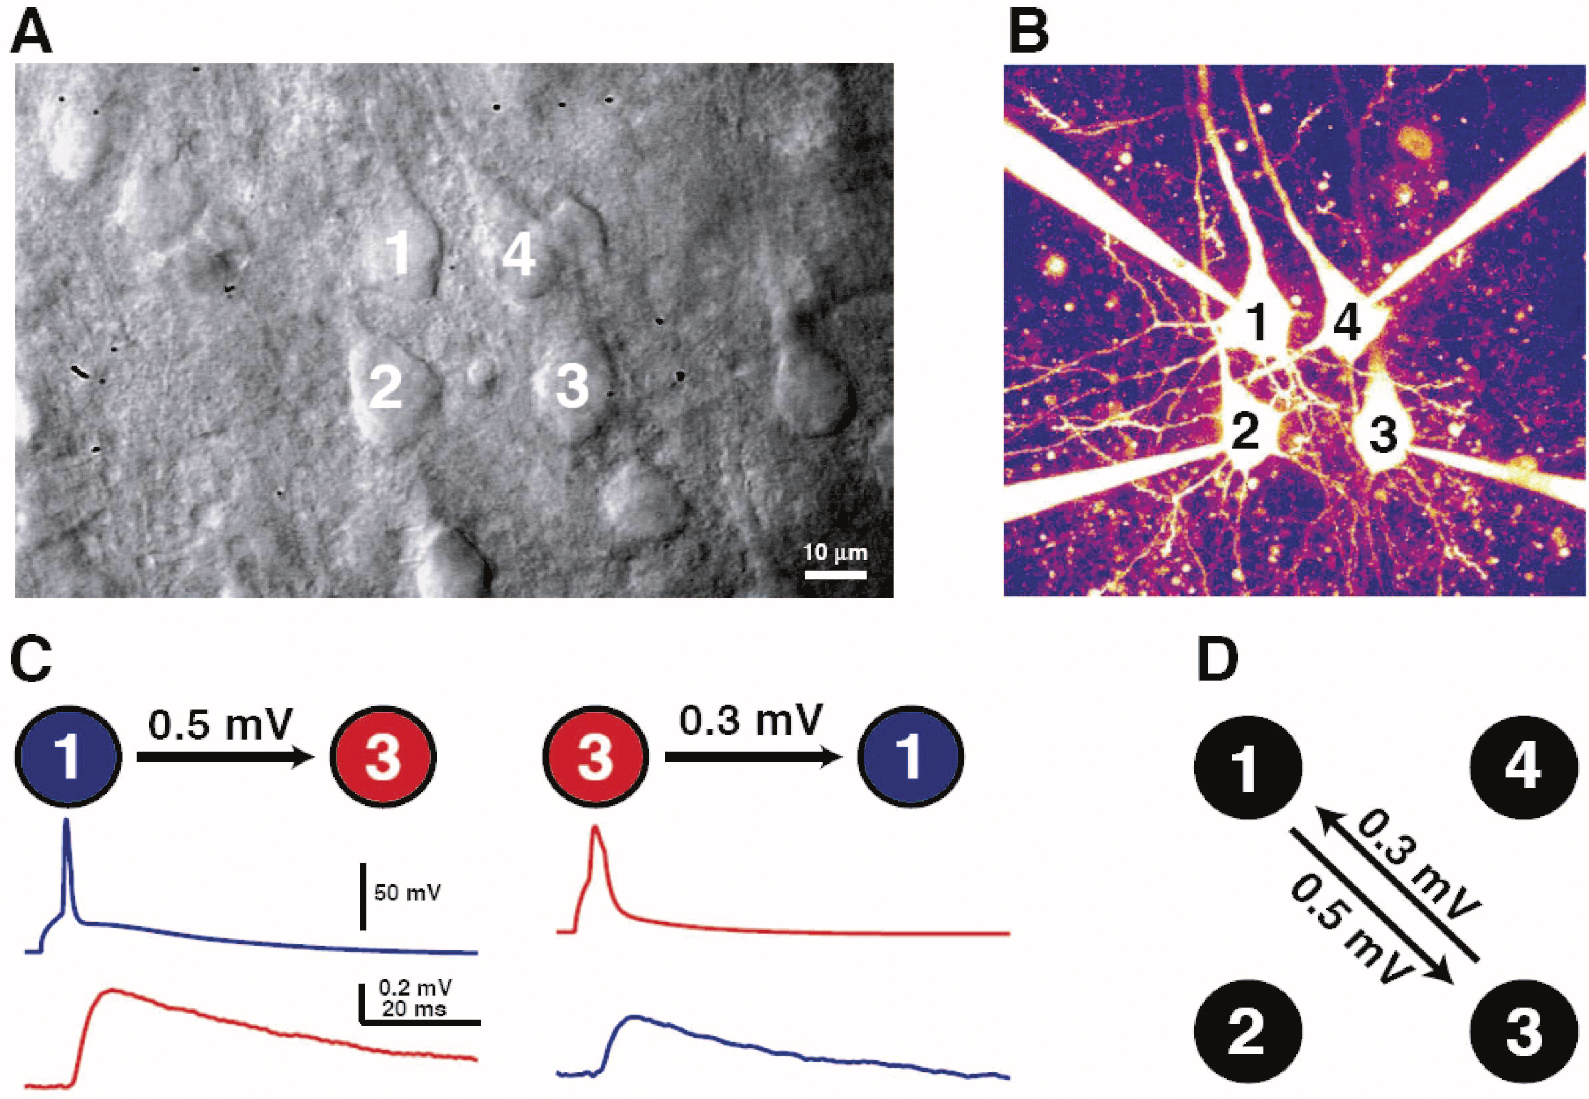
\includegraphics[width=.75\linewidth]{img/song2005-quadruplet_recordings.png}
  \caption{Song et al. use quadruple whole-cell recordings, observing
    simultaneously the membrane potential of four neurons.
    \textbf{A)} Contrast image showing four thick-tufted L5 neurons
    \textbf{B)} Fluorescent image of the same cells after patching on
    \textbf{C)} Evoking an action potential in the presynaptic neuron
    causes characteristic membrane potential change in the
    postsynaptic neuron \textbf{D)} Infering synaptic connectivity
    from the EPSP waveform observed in C). Image from \textcite{Song2005}.
    % \texttt{\textcolor{linkgrey}{3b056efe-3ebc}}
  }
\end{figure}
%\vspace{0.45cm}

While techniques for paired intracellular recordings are rapidly
developing, their ability to capture connectivity patterns of large
networks is yet very limited. To this date, the connectome of
\textit{C. Elegans} remains the outstanding exception of a
connectivity configuration that has been fully mapped
\parencite{White1986}. Even in the state-of-the-art experiment
conducted by Perin et al., using a setup capable of recording up to
twelve neurons simultaneously, the authors note that an investigation
of degree distribution was not carried out, due to lack of sufficient
data
\parencite{Perin2011}.

Working with a geometrical network model and its computational
\marginpar{exploiting the benefits of a geometrical model}
implementation, such restrictions disappear; the full information
about the network, in form of its connectivity matrix, is given at
point in time and can be easily queried for. Experiments that may take
days to perform \textit{in vivo}, can be completed in a matter of
seconds \textit{in silico}. As such, geometrical models lend
themselves to extensive examination of their structural aspects.  In
trying to exploit these advantages, two approaches present
themselves. One may construct a network model that extrapolates the
known biological configuration; a full structural examination of these
networks could possibly expose relevant patterns not yet observed. For
this approach a sophisticated understanding of the biological
configuration is critical. Neuron morphology, however, is difficult to
describe and extract. For this analysis we suggest a reductionist
approach. Having motivated an abstract model reflecting a cortical
network's anisotropy in connectivity, we distinguish emerging
structural patterns, specific to anisotropic networks, from results,
that only indirectly stem from the network's anisotropy, in the hopes
to be able to characterize the significance of directional
heterogeneity in structural connectivity of cortical circuits.


In this chapter we subject the anisotropic network model introduced in
Section~\ref{sec:anisotropic_network_model} to a critical analysis of
its structural aspects. General network topology, as well as specific
modes and patterns of connectivity, are to be identified and laid out
for comparison with findings in biological neural networks.  In an
effort to identify structural features that can be directly associated
with the network's anisotropy in connectivity, \marginpar{rewired and
  \mbox{distance-depen}\-dent networks as reference} it is crucial to
differentiate such findings from results that are only indirectly
caused by the network's anisotropy. To this end we are recruiting the
different network types introduced in the previous chapter throughout
this analysis. Having shown a decreasing degree of anisotropy in
rewired and distance-dependent networks, both models will serve as
reference to compare against for structural features found in
anisotropic networks. Analyzing standard graph measures in the first
two sections, we quickly move on to towards neuronal network specific
connectivity and anisotropy's role in being able to model such highly
non-random patterns in the later sections.


% ######################################################################### %
% ------------------------------------------------------------------------- %
%                             Comment Stuff
% ------------------------------------------------------------------------- %
% ######################################################################### %


% Human Connectome Project and the Open Connectome Project, the
% continued development of experimental techniques and of resources
% like the Brain Connectivity Toolbox software, as well as the
% research of theoreticians and experimentalists, are all dedicated
% towards the common goal of charting brain connectivity.

% In this general sense, brain connectivity can refer to linking
% between distinct units at various scales. From the mapping of fiber
% pathways between brain regions on the macroscale, to the synaptic
% connections of individual neurons on the microscale,
% [\textcolor{linkgrey}{Scholarpedia}].

% It is interesting not only to investigate for anatomical
% connections, but functional and causal as well. However, exploring
% the aspects of our specific geometric network model, in this chapter
% the connectivity of interest to us is the structural connectivity at
% the microscale, that is synaptic connections between individual
% neurons.

% \marginpar{Human Connectome Project
% \mbox{\url{humanconnectome.org}}}

% \parbox{1.8cm}{Human Connectome
% Project}
\includegraphics[width=0.45\linewidth]{img/HCP_logo.png}
% \mbox{\url{humanconnectome.org}}}


% Ho Ko connectivity -> specific dynamics.
% Pernice -> Spike Train Correlations. Maybe Shepherd 2005?

% ...and have been linked to brain function and dynamics.

% *What cool things synaptic connectivity does.  , stores memory, drives
% dynamics, etc.  While brain is plastic, there is structure that is
% believed to provide a framework, boundary conditions to

% *patterns of synaptic connectivity is neither completely random nor
% exclusively specific, patterns emerge [Sporns, Perin, Song]
 
% This specific, non-random connectivity largely impact dynamics and
% brain function:


% Connectivity in the directionally heterogenous geometric networks
% introduced in ??, models synaptic contacts between axon and
% dendrites of individual neurons. In this chapter

% It is then the task of this theoretical framework to provide results
% interesting to the biological situation. An investigation on how well
% an introduced model can reproduce certain structural aspects of
% networks that have already been fund is integral to the study of a
% computational model. But, furthermore, a model should aspire to
% extrapolate results found in the biological
% situation.



%%% Local Variables: 
%%% mode: latex
%%% TeX-master: "../dplths_document"
%%% End: 

% \newpage
% \input{Chapters/072_}

%Hell


% radius of the bulk spectrum


% % 80%-20%

% Inhib synapse








%%% Local Variables: 
%%% mode: latex
%%% TeX-master: "../dplths_document"
%%% End: 
